\documentclass{article}
\usepackage[utf8]{inputenc}
\usepackage{amsmath}
\usepackage{graphicx}

\title{Relazione}
\author{Tommaso De Nicola 2006686}
\date{Giugno 2022}

\begin{document}

\maketitle

\centering

\section{Introduzione}
Il progetto "Forza Quattro" consiste nel implementare in Java il medesimo gioco sfruttando le interazioni tra oggetti come l'ereditarietà o polimorfismo (progetto per console).


\section{Descrizione delle classi}
Nell'implementazione effettuata sono presenti 5 classi totali.


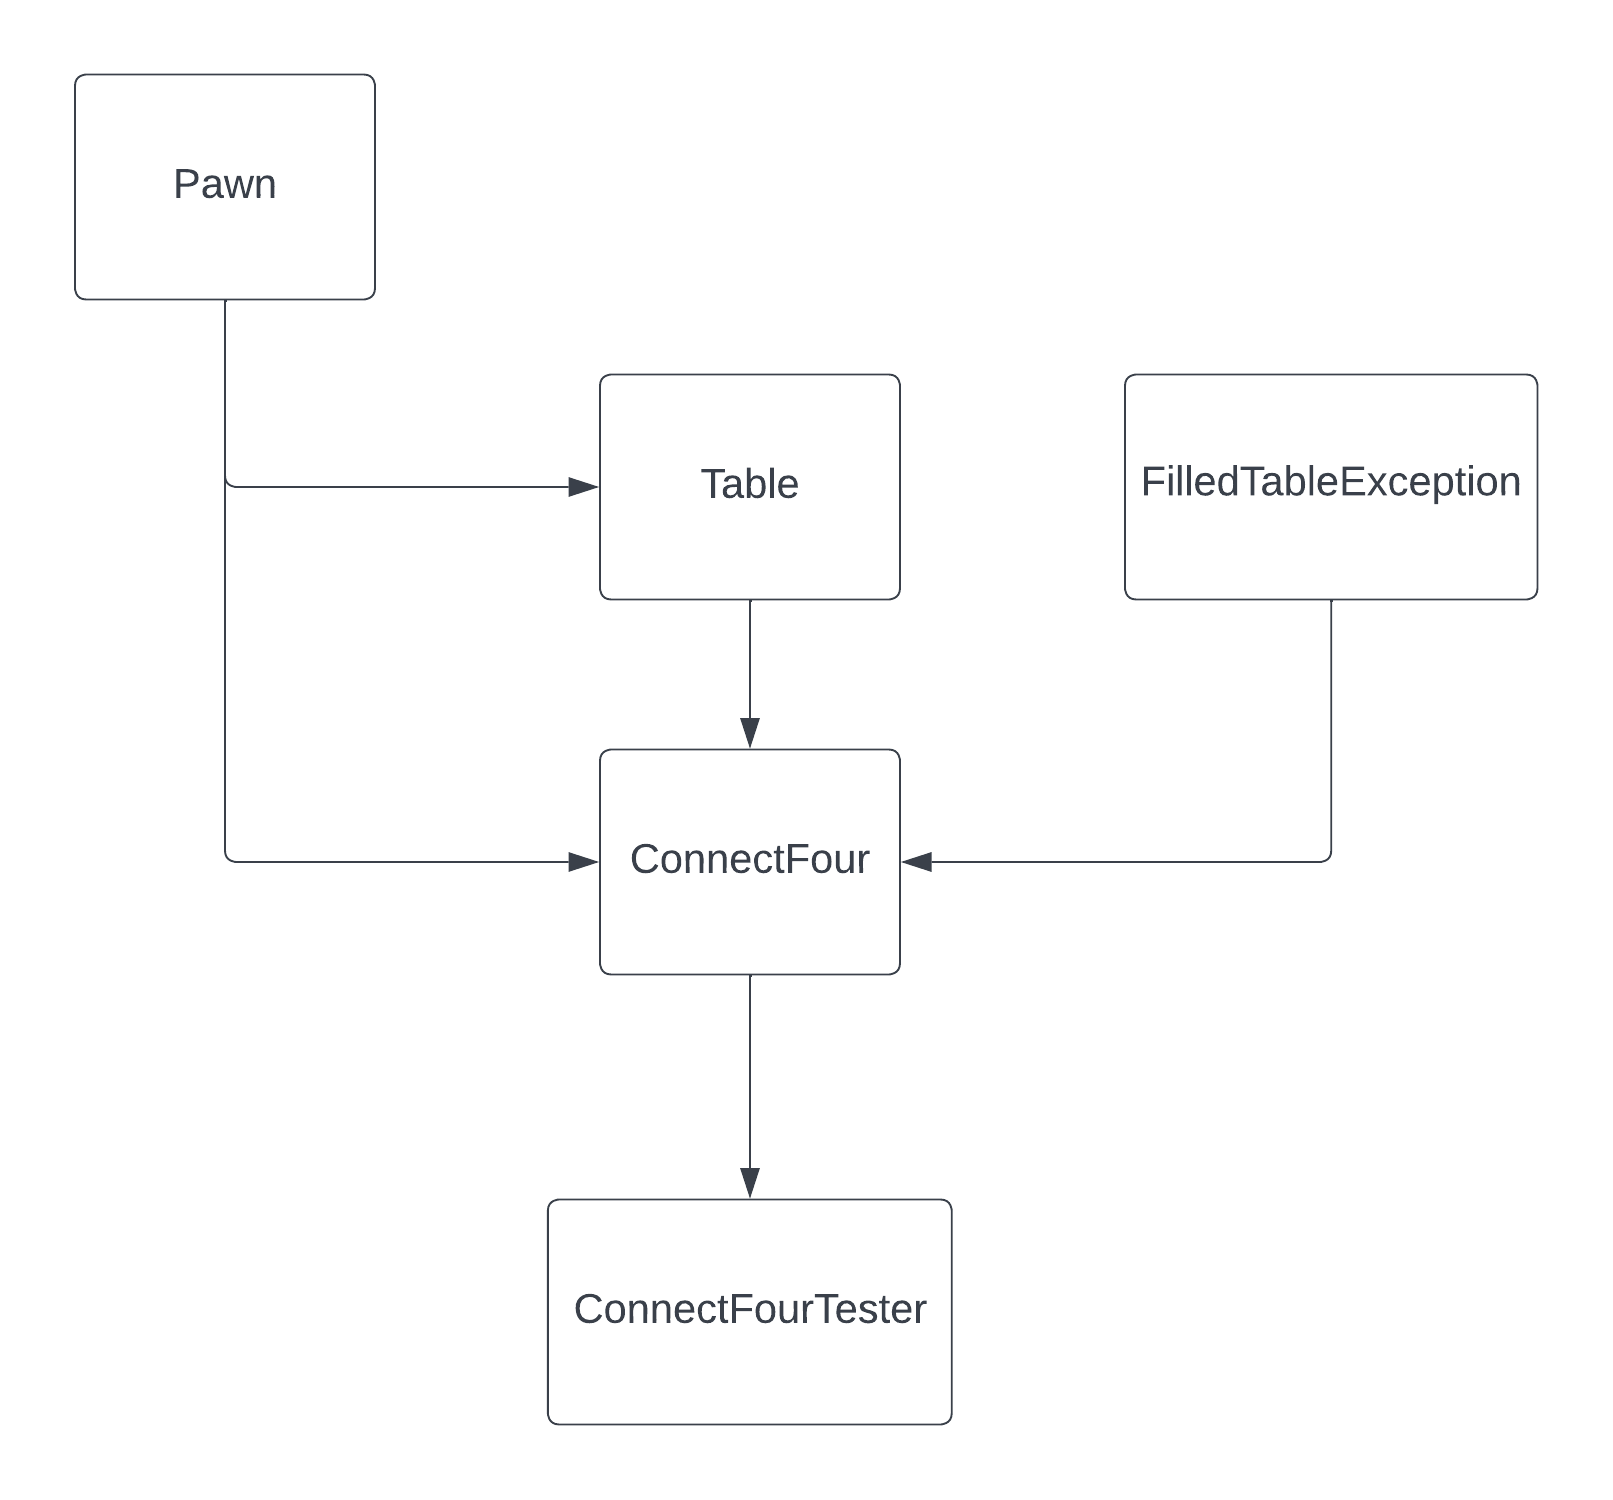
\includegraphics[width=0.7\textwidth]{uml.png}


\subsection{Pawn}
la classe di base è l'oggetto "Pawn" che rappresenta la pedina di gioco con correlato colore rappresentativo con i rispettivi metodi per impostare, prelevare e resettare il carattere della pedina e il colore.


\subsection{Table}
La classe "Table" utilizza la classe "Pawn" al suo interno realizzandone una tabella con possibilità di impostarne la dimensione e impostare le pedine dei giocatori durante l'inizializzazione, di poter aggiungere una pedina di un giocatore nella corrispettiva casella selezionata; infine è anche possibile reimpostare la tabella svuotandola


\subsection{FilledTableException}
Rappresenta una versione rivisitata della classe Exception, utilizzata in caso di inserimento di una pedina in una tabella piena.


\subsection{ConnectFour}
Essa è la classe cardine del programma, poiché rappresenta in maniera vera e propria il gioco di forza quattro.

Essa Inizializza una nuova tabella (super classe) di dimensione 6x7 e con rispettivamente 2 giocatori con rispettive pedine e colori.

Presenta anche una vasta varietà di metodi quali la versione soggetta ad override dell'aggiunta della pedina che riprende dalla classe padre il metodo con l'aggiunta di dell'effetto gravità alle quali sono soggette le pedine; in caso di colonna piena ritornerà un errore all'utente o, in caso di mappa piena terminerà il gioco.

Sono presenti anche metodi necessari quali il controllo della vittoria, per controllare l'eventuale vittoria del giocatore corrente, e il metodo di gioco che ci permetterà di continuare la partita in maniera ciclica con ristampa a video della tabella di gioco ogni turno.

Infine abbiamo dei metodi di contorno per migliorare l'esperienza di gioco che introducono un menù con corrispettivo comando per chiedere aiuto, e metodi per salvare la partita corrente dandole un nome, e quello per caricare una precedente partita sospesa identificata con il nome del salvataggio precedentemente inserito.


\subsection{ConnectFourTester}
La classe addetta a far iniziare il gioco inizializzando "ConnectFour".


\section{Descrizione delle funzionalità}
Il gioco una volta fatto partire, si presenterà come una console, in ogni menù e sottomenù è presente il comando "help" che se lanciato stamperà a schermo la lista di comandi del menù corrente con eventuali argomenti.

Appena avviato il programma avremo la possibilità di uscire con "exit" o "quit", iniziare una nuova partita con "start" o "new", oppure continuare un partita messa in pausa precedentemente con "continue" o "load" seguito dal nome del salvataggio.

Una volta avviata una partita ci troveremo in un sottomenù dal quale si potrà uscire con "exit" o "quit"; per giocare basterà inserire il numero della colonna nella quale si vuole inserire la propria pedina, il turno si alterna ogni mossa automaticamente andando a chiedere al giocatore di turno ciò che si vuole fare.
Infine è possibile salvare ed interrompere la partita con "pause" o "save" seguito dal nome che si vuole dare al salvataggio (in caso di nome identico ad un precedente salvataggio, verrà sovrascritto).

La partita si conclude quando uno dei giocatori posiziona 4 pedine consecutive in orizzontale, verticale o diagonale, oppure quando la tabella è completamente piena e non si può procedere con la partita concludendola in parità.


\end{document}
